\documentclass[]{thesis-ekf}
\usepackage[T1]{fontenc}
\PassOptionsToPackage{defaults=hu-min}{magyar.ldf}
\usepackage[magyar]{babel}
\usepackage{mathtools,amssymb,amsthm,pdfpages}
\footnotestyle{rule=fourth}

\newtheorem{tetel}{Tétel}[chapter]
\theoremstyle{definition}
\newtheorem{definicio}[tetel]{Definíció}
\theoremstyle{remark}
\newtheorem{megjegyzes}[tetel]{Megjegyzés}

\begin{document}

\institute{Matematikai és Informatikai Intézet}
\title{PokerParty}
\author{Szabó Márk\\programtervező informatikus Bsc.}
\supervisor{Troll Ede\\tanársegéd}
\city{Eger}
\date{2025}
\maketitle

\tableofcontents

\chapter*{Bevezetés}
\addcontentsline{toc}{chapter}{Bevezetés}

\chapter{Technológiai áttekintés}

\section{Enginek}
Általános leírás és összehasonlítás az API alapú fejlesztéssel

\subsection{Unreal}
\subsection{Godot}
\subsection{Unity}

\section{Többjátékos technológia a játékfejlesztésben}

\subsection{Korai megoldások}
Helyi többjátékos mód
\subsection{Kliens-Szerver}
\subsection{Dedikált szerver}
\subsection{Peer-to-Peer (P2P)}

\chapter{Rendszerterv}
Azok az elemek, amiket tanultatok RFT-n, azok kerülnek ide

\section{Rendszer célja}
\section{Követelmények}
\section{Architekturális terv}
PC unity, Mobile unity, SharedDLL
\section{Használt fejlesztői eszközök}

\chapter{Saját szoftver megvalósítása}

\section{Többjátékos kapcsolat megvalósítása}

\subsection{Kapcsolat kezelése a PC oldalon}
\subsection{Kapcsolat kezelése a Mobile oldalon}

\section{Texas Hold'Em}

\subsection{Bevezetés}

A póker a világ egyik legismertebb kártyajátéka, amelyben a játékosok célja, hogy a saját lapjaikból a lehető legjobb kombinációt kialakítva megszerezzék az asztalon lévő kasszát. A póker számos különböző szabályrendszerrel rendelkező változatban létezik.

A \emph{Texas~Hold’Em} a közösségi pókerjátékok legnépszerűbb formája, amelyet jellemzően 2 és 10 játékos között játszanak. Ez egy viszonylag zárt struktúrájú játék, ahol a licitálás menete állandó szabályok szerint zajlik.

\subsection{Szabályok ismertetése}

A házi vagy baráti társaságokban játszott póker esetében a szabályok gyakran eltérhetnek, mivel a játékosok igyekeznek a saját ízlésük szerint alakítani azokat, hogy még élvezetesebb legyen a játék. Ebben a fejezetben a póker legelterjedtebb, hivatalos versenyeken is alkalmazott szabályrendszere kerül bemutatásra. Ami közös az összes variációban, hogy a játékot 52~lapos francia kártyával játsszák dzsókerek nélkül.

\subsubsection{A játék menete \cite{WikipediaTexasholdem}}

A játék során három fontos szerep forog körbe a játékosok között, amit ,,gombokkal'' jelölünk. Ezek a szerepek az osztó, kis vak és nagy vak. Az osztótól balra ülő játékos lesz a kis vak, a kis vaktól balra ülő pedig a nagy vak. Az osztót pedig több különböző módon választhatjuk meg a játék elején.  

Az osztó keveri és osztja ki a lapokat a szabályok szerint. A vakok pedig még osztás előtt kötelesek betenni a vak téteket, ahol a kis vak tét általában a nagy vak tét fele.

\begin{enumerate}
	\item \emph{Osztás}
	\begin{itemize}
		\item Az osztó először megkeveri a paklit. A kiosztás előtt a kis vak és a nagy vak beteszik a kötelező téteket. Ezt követően az osztó balról kezdve, két körben, egyesével oszt minden játékosnak egy-egy zárt lapot.
	\end{itemize}
	\item \emph{Pre-Flop (első licitkör)}
	\begin{itemize}
		\item A licitálás a nagy vaktól balra ülő első játékossal kezdődik, aki az alábbi lehetőségek közül választhat:
		\begin{itemize}
			\item Tartás -- megadja az aktuális tétet.
			\item Emelés -- növeli a tétet a limitszabályok szerint.
			\item Dobás -- eldobja a lapjait, ezzel kiszáll a játékból.
		\end{itemize}
		\item A licitálás az óramutató járásával megegyező irányban halad tovább.
		\end{itemize}
	\item \emph{Flop (második licitkör)}
	\begin{itemize}
		\item Az osztó egy lapot félretesz égető lapként, majd három közös lapot felfordítva az asztal közepére helyez.
		\item A licitálást az osztógombtól balra ülő első aktív játékos kezdi, és az alábbi lehetőségek közül választhat:
		\begin{itemize}
			\item Passzolás -- nem emel, de marad a játékban.
			\item Nyitás -- tétet tesz be a limitszabályok szerint.
			\item Dobás -- eldobja a lapjait és kiszáll a körből.
		\end{itemize}
		\item Ha valaki nyit, a többiek dönthetnek:
		\begin{itemize}
			\item Tartás -- megadják a tétet.
			\item Emelés -- növelik a tétet.
			\item Dobás -- kiszállnak a körből.
		\end{itemize}
	\end{itemize}
	\item \emph{Turn (harmadik licitkör)}
	\begin{itemize}
		\item Az osztó ismét éget egy lapot, majd egy negyedik közös lapot felfordítva az asztalra helyez.
		\item A harmadik licitkör a második licitkörhöz hasonlóan zajlik.
	\end{itemize}
	\item \emph{River (negyedik licitkör)}
	\begin{itemize}
		\item Az osztó még egy égető lapot félretesz, majd kiosztja az utolsó, ötödik közös lapot.
		\item Minden játékos hét lapból próbálja a lehető legjobb ötlapos kombinációt kialakítani.
		\item Az utolsó licitkör a második és a harmadik licitkörhöz hasonlóan zajlik.
	\end{itemize}
	\item \emph{Showdown (lapok felfedése)}
	\begin{itemize}
		\item Ha az utolsó licitkör után egynél több játékos marad, akkor a játékosok megmutatják a lapjaikat választásuk szerint.
		\item A kasszát a legerősebb pókerkezet birtokló játékos nyeri el.
	\end{itemize}
\end{enumerate}

\subsubsection{A pókerkezek \cite[9.~oldal]{Szurdi}}

Az alábbi felsorolás a lehetséges pókerkezeket mutatja be, amelyeket erősségük szerint rendeztem el, a legerősebbtől a leggyengébbig. A lista tetején található kéz a pókerben elérhető legmagasabb értékű kombináció, és innen lefelé haladva egyre gyengébb kezek következnek. Az alábbi sorrendet megtekinthetjük \aref{fig-pokerhands}.~ábrán is. 

\begin{enumerate}
	\item \emph{Royal flös (royal flush)}
	\begin{itemize}
		\item A legerősebb lapkombináció. Egyszínű 10-es, bubi, dáma, király, ász lapokból áll. Ha két ilyen találkozik, akkor döntetlen\footnote{Osztozás történik a nyeremény között.} van.
	\end{itemize}
	\item \emph{Színsor (straight flush)}
	\begin{itemize}
		\item Öt egyszínű sorba rendezhető lapból áll. Ha két ilyen találkozik, a legmagasabb lap dönt. Ha egyforma, akkor döntetlen van. 
	\end{itemize}
	\item \emph{Póker (four of a kind)}
	\begin{itemize}
		\item Négy ugyanolyan számozású vagy jelű lapból és egy akármilyen másik lapból áll. Ha két ilyen találkozik, a magasabb póker nyer.
	\end{itemize}
	\item \emph{Full (full house)}
	\begin{itemize}
		\item Három ugyanolyan számozású vagy jelű lapból és két másik ugyanolyan számozású vagy jelű lapból áll. Ha két ilyen találkozik, a magasabb drill nyer. Ha egyforma, a magasabb pár nyer.
	\end{itemize}
	\item \emph{Szín (flush)}
	\begin{itemize}
		\item Öt ugyanolyan színű lapból áll. Ha két ilyen találkozik, a legmagasabb lap dönt. Ha egyforma, a második legmagasabb dönt, és így tovább\dots
	\end{itemize}
	\item \emph{Sor (straight)}
	\begin{itemize}
		\item Öt sorba rendezhető lapból áll. Ha két ilyen találkozik, a legmagasabb lap dönt. Ha egyforma, a színerősség dönt.
	\end{itemize}
	\item \emph{Drill (three of a kind)}
	\begin{itemize}
		\item Három ugyanolyan számozású vagy jelű lapból és két akármilyen másik lapból áll. Ha két ilyen találkozik, a magasabb drill nyer. Ha egyforma, a magasabb semleges lap, majd az alacsonyabb dönt.
	\end{itemize}
	\item \emph{Két pár (two pairs)}
	\begin{itemize}
		\item Kétszer két ugyanolyan számozású vagy jelű lapból áll. Ha két ilyen találkozik, a magasabb pár, majd az alacsonyabb, majd a semleges lap erőssége dönt.
	\end{itemize}
	\item \emph{Egy pár (one pair)}
	\begin{itemize}
		\item Két ugyanolyan számozású vagy jelű lapból és három akármilyen másik lapból áll. Ha két ilyen találkozik, a magasabb pár nyer. Ha egyforma, a semleges lapok döntenek.
	\end{itemize}
	\item \emph{Magas lap (high card)}
	\begin{itemize}
		\item Bármilyen lap, abból is a legmagasabb értékkel rendelkező.
	\end{itemize}
\end{enumerate}

\begin{figure}[ht!]
	\centering
	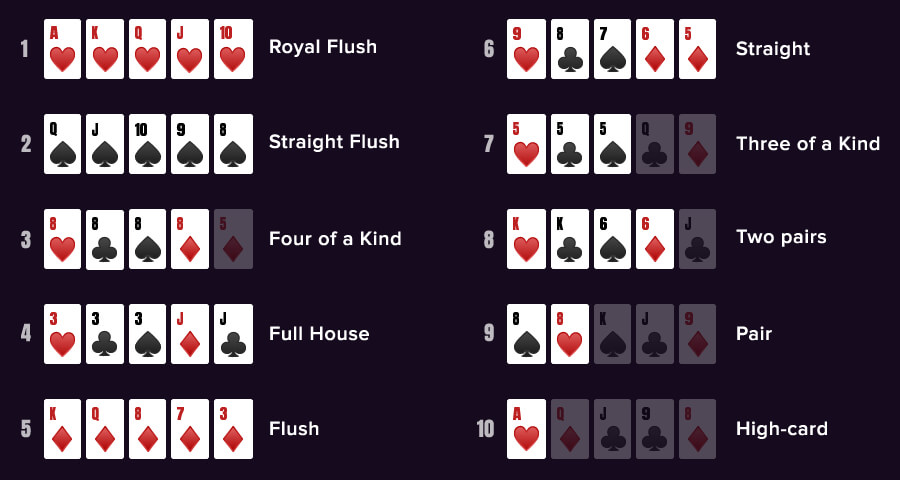
\includegraphics[width=12cm]{poker_hands}
	\caption{Lehetséges pókerkezek}
	\label{fig-pokerhands}
\end{figure}

\subsection{Használt kézkiértékelő algoritmus}

A legelterjedtebb kézkiértékelő algoritmusok azon alapulnak, hogy a kezek értékeit egy előre kiszámított kéz értékeket tároló táblából keressük ki. Ez az egyik leggyorsabb módszer, viszont a módszer egy nagy hátránya a nagy méretű tábla tárolása, amely tárhely igényes. A játékomban egy bit matematikán alapuló algoritmust használtam, aminek alapjait \acite{HandEvaluation} blog adta. Ez a módszer lassabb, mint a táblás, viszont a tárhely igényes probléma itt megszűnik.

\subsubsection{Az algoritmus}

Minden kártyáról tároljuk a számozását és a színét. Az input 5 darab ilyen kártyából fog állni.

\begin{enumerate}
	\item 2 különböző bit mező létrehozása a kártyák alapján
	\begin{itemize}
		\item első mező
		\item második mező
	\end{itemize}
	\item kéz értékelés a második bit mező segítségével
	\item sorok ellenőrzése
	\item flush ellenőrzése
	\item döntetlenek eldöntése
\end{enumerate}



\section{Játékmenet megvalósítása}

\subsection{Modul1}
\subsection{Modul2}

\chapter{Tesztelés}

\section{SharedDLL tesztelése}
\section{PC játék tesztelése}
\section{Mobile játék tesztelése}
\section{Általános tesztelés}

\chapter*{Összegzés}
\addcontentsline{toc}{chapter}{Összegzés}

\begin{thebibliography}{2}
	\addcontentsline{toc}{chapter}{\bibname}
	\bibitem{WikipediaPoker}
	\textsc{Wikipedia}: \emph{Póker}, Wikipedia, az online enciklopédia, elérhető: \url{https://hu.wikipedia.org/wiki/P%C3%B3ker} [Letöltve: 2024-11-12]
	\bibitem{WikipediaTexasholdem}
	\textsc{Wikipedia}: \emph{Texas Hold'Em}, Wikipedia, az online enciklopédia, elérhető: \url{https://hu.wikipedia.org/wiki/Texas_Hold%E2%80%99Em} [Letöltve: 2024-11-13]
	\bibitem{HandEvaluation}
	\textsc{Jonathan Hsiao}: \emph{Evaluating Poker Hands with Bit Math}, Jonathan Hsiao blogja, elérhető:: \url{https://jonathanhsiao.com/blog/evaluating-poker-hands-with-bit-math} [Letöltve: 2025-02-25]
	\bibitem{Szurdi}
	\textsc{Szurdi András}: \emph{Pókerkönyv. Kezdőknek és haladóknak}, Ciceró, Budapest, 1995.
	\bibitem{Varga}
	\textsc{Varga Ervin}: \emph{Póker alapkönyv}, Vagabund, Kecskemét, 2008.
\end{thebibliography}

% Aláírt, szkennelt nyilatkozat beillesztése a szakdolgozat végére
%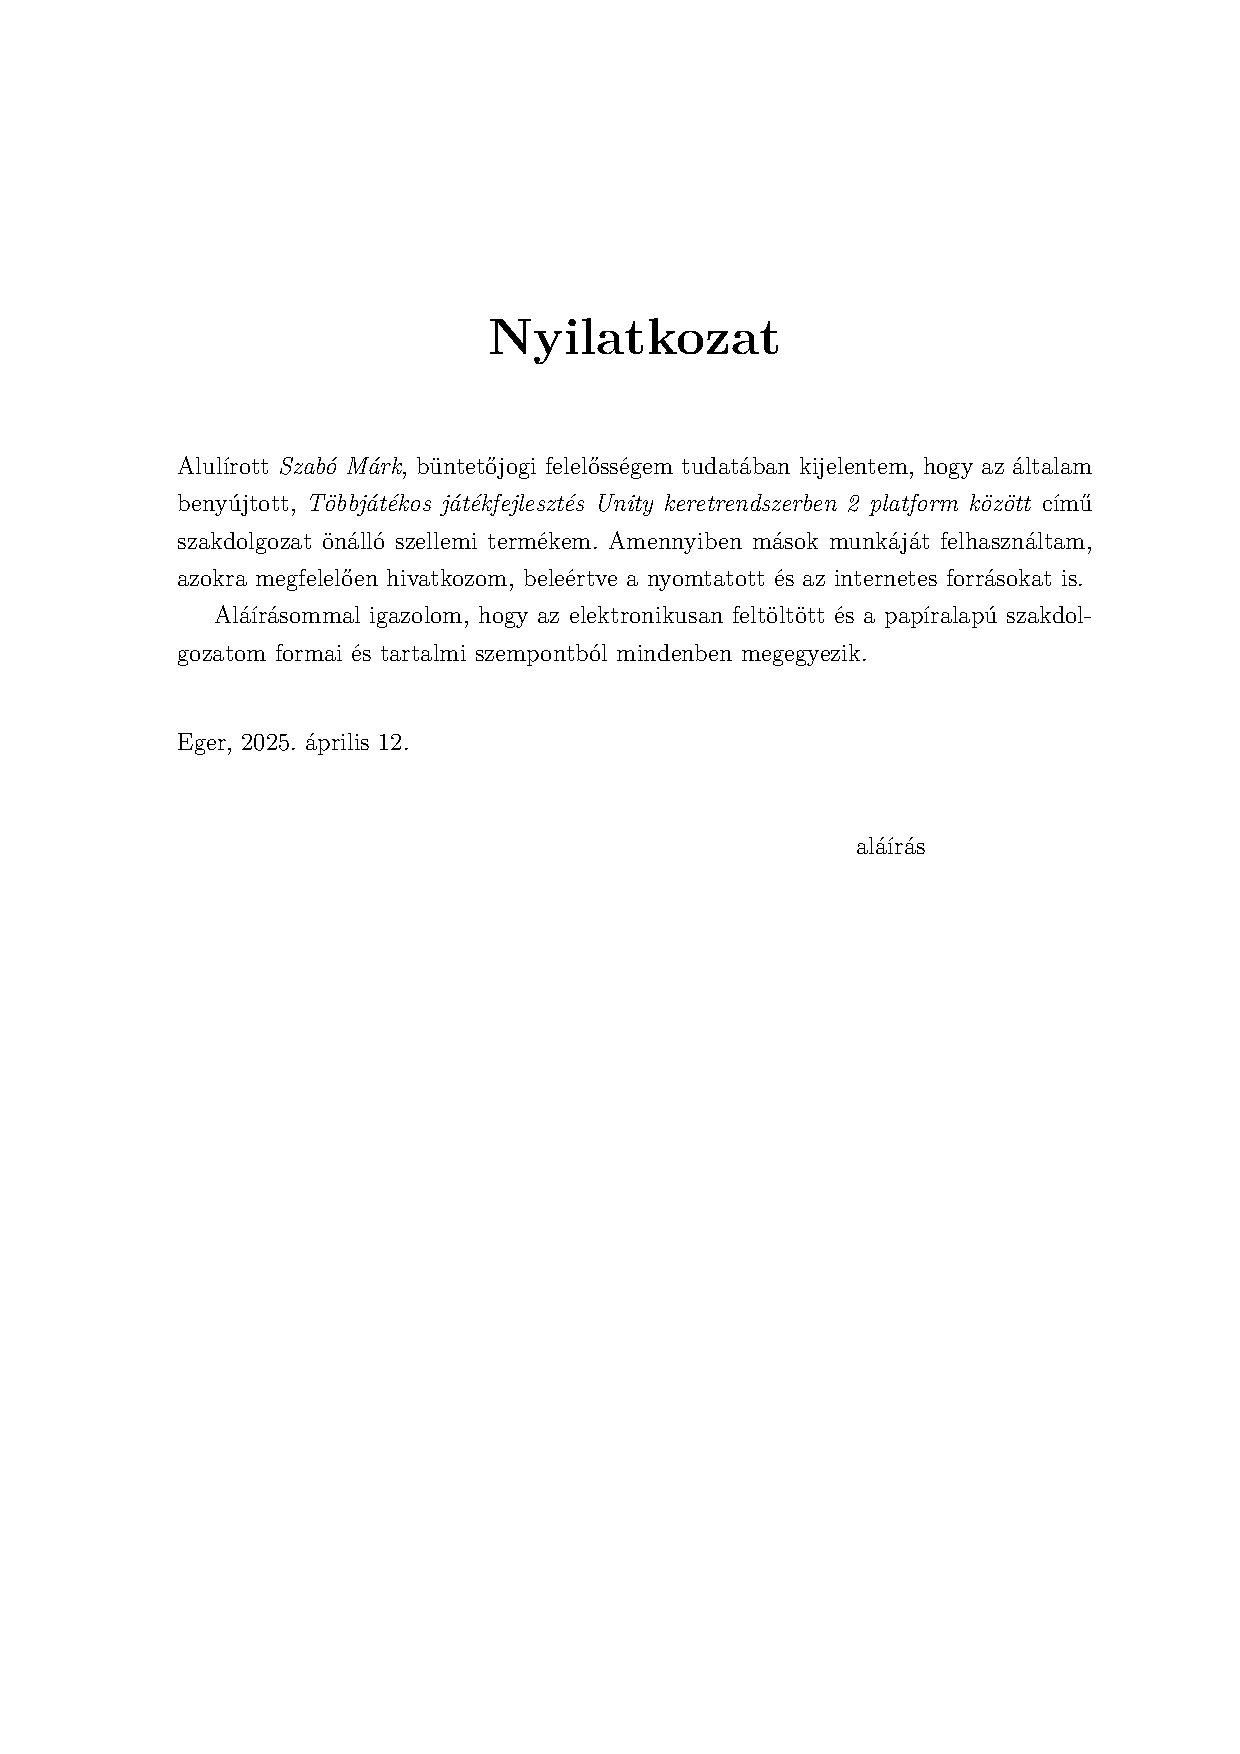
\includepdf{nyilatkozat/nyilatkozat.pdf}
\end{document}